\documentclass[conf]{new-aiaa}
%\documentclass[journal]{new-aiaa} for journal papers
\usepackage[utf8]{inputenc}

\usepackage{graphicx}
\usepackage{amsmath}
\usepackage[version=4]{mhchem}
\usepackage{siunitx}
\usepackage{longtable,tabularx}
\setlength\LTleft{0pt} 
\usepackage{multirow}
\usepackage{float}


\title{Optimization of Look-Ahead controller gains for simulation of autonomous vehicle path-tracking}

\author{O. Elsewify\footnote{Master's Student, Mechanical Engineering, 440 Escondido Mall Building 530, Stanford, CA 94305} and A. Mhish\footnote{Master's Student, Mechanical Engineering, 440 Escondido Mall Building 530, Stanford, CA 94305}}
\affil{Stanford University, Stanford, CA, 94305}

\begin{document}

\maketitle

\begin{abstract}
In this paper a design approach is presented for the optimization of the controller gains of a Look-ahead controller for an autonomous vehicle. When implemented, the resulting controller must ensure that the system can follow a fixed trajectory, at a desired speed profile, within a set range of lateral and longitudinal accelerations. The problem is a multi variable optimization problem, with three controller gains as the desired output.
Several optimization approaches are considered and performance of the algorithms are evaluated and compared.
\end{abstract}

\section{Nomenclature}

{\renewcommand\arraystretch{1.0}
\noindent\begin{longtable*}{@{}l @{\quad=\quad} l@{}}
$K_{LA}$ & look-ahead gain \\
$x_{LA}$ & look-ahead distance (m)\\
$K_{long}$& longitudinal gain \\
$\delta$ & steering angle (rad)\\
$F_{x}$ & longitudinal force (N) \\
$e$ & lateral error at CG (m)\\
$\Delta U_x$ & longitudinal vehicle velocity error (m/s)\\
$a_x$ & longitudinal acceleration (m/$s^2$)\\
$a_y$ & lateral acceleration (m/$s^2$)\\
$x$ & design variable \\
$f$ & general function \\
$f_{obj}$   & objective function\\
$c$  & constraints \\
$\alpha$ & step size\\
$\rho$   & initial penalty \\
$\gamma$ & penalty multiplier\\
\end{longtable*}}

\section{Introduction}
In the world of controllers, one of the most interesting topics is the topic of path tracking for autonomous vehicles. The objective is to be able to follow a predetermined trajectory and speed profile as closely as possible, using sensors to gather information and a controller and actuators to determine required steering angle and acceleration. There exist several controller types which effectively serve this purpose, each of which undoubtedly requires some degree of tuning and optimisation, there are no off-the-shelf controllers that work for all problems. 

It is the role of control engineers to determine the appropriate parameters (gains) that allow the controller to complete its task effectively. In the past, engineers would be required to generate several control diagram plots including Root-Locus, Nyquist, and Bode, all of which would provide them with a general idea as to what gains should be tested. The typical process for testing and validation of controllers in the physical world can be time consuming and expensive, placing a strong emphasis on the design of an accurate and robust controller before implementation.

With the advent of numerical modeling and simulation, engineers are now able to test and develop their designs in the virtual world at much lower costs. Engineers can iterate through their design parameters hundreds of thousands of times per minute, track improvement in their designs, and finally select the optimal solution to the problem. Furthermore, the computational power of modern machines allow for advanced analysis of large data sets revealing hidden trends in the data that otherwise would go unnoticed.

\section{Vehicle Dynamics and Control Theory}
An ideal controller is designed around two requirements: integrated longitudinal and lateral control, and robustness against noisy inputs \cite{bayuwindra2019look}. The lateral control part of the look-ahead controller takes instantaneous heading error $\Delta\psi$, lateral error $e$, and longitudinal velocity $U_x$ as inputs and returns a steering angle $\delta$ which will point the vehicle towards the path. This relationship can be summarised by the following equation:
\[\Delta\psi_{ss}=\kappa(\frac{maU_x^2}{LC_{{\alpha}r}}-b)\]
\[\delta_{ff}=\frac{K_{LA}x_{LA}}{C_{{\alpha}f}}\Delta\psi_{ss} + \kappa(L+KU_x^2)\]
\[\delta=-\frac{K_{LA}}{C_{{\alpha}f}}(e+x_{LA}\Delta\psi)+\delta_{ff}\]

The second part of the controller involves the control of longitudinal velocity $U_x$, the equivalent of pressing the accelerator pedal.

\begin{figure}[hbt!]
\centering
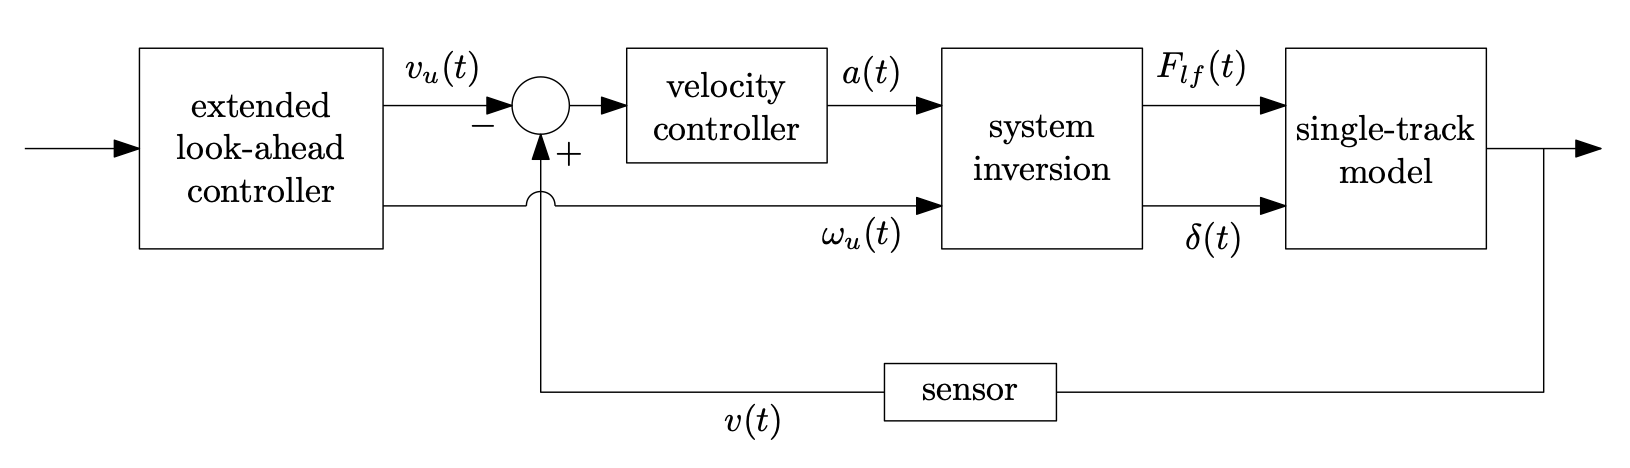
\includegraphics[width=0.75\textwidth]{lookahead_fb}
\caption{Block diagram of the look-ahead controller with integrated longitudinal velocity feedback control\cite{bayuwindra2019look}}
\end{figure}

\section{Optimization Approach}
This paper looks at the iterative design approach for a Look-Ahead controller. The objective of this paper is to develop a robust algorithm that can use an existing data set containing design variables $\textbf{x} \in \mathbb{R}^3$:
\begin{center}
\textbf{x} = [$K_{LA}$    $x_{LA}$  $K_{long}$]
 \end{center}
and their respective simulation results $y($\textbf{x}$)$ $\in \mathbb{R}^4$
 \begin{center}
$y(\textbf{x})$ = [$e$    $\Delta U_{x}$  $a_y$   $a_x$]
 \end{center}
to accurately predict the results for any given $\textbf{x}$. Once this regression model for the function $f$ has been established it is then possible to optimise the for the ideal design variable $x^*$. 
 
The resulting $x^*$ containing the ideal controller gains is then tested in the virtual MATLAB simulation environment and the results are collected and compared against the existing data-set to measure improvement on the existing data samples.

\subsection{Constraints}

There are four main design constraints \textbf{g}(\textbf{x)} imposed on this problem, the first of which is a constraint on the allowable lateral error $e$. The further the vehicle center of gravity is to the left or right of the desired trajectory the larger the error. As such it is best ensure that the lateral error is kept to a minimum, in this problem the allowable lateral error is 20 cm.
\[e\leq0.20\]
The second constraint is on the error in longitudinal velocity tracking $\Delta U_x$. The greater the deviation in the instantaneous velocity from the desired velocity on the speed profile the greater the magnitude of longitudinal velocity error. In this problem the maximum allowable $\Delta U_x$ is 0.75 m/s.
\[\Delta U_x\leq0.75\]
Furthermore, both the maximum lateral and longitudinal accelerations are constrained, such as to reduce the jerkiness motion of the vehicle. A reasonable value of 4 $m/s^2$ is selected for this problem. This constraint is imposed on both the negative (braking) and positive (accelerating) acceleration directions.
\[|a_y|\leq4\]
\[|a_x|\leq4\]

\subsection{Cost Function}

The cost function designed for this problem is designed with the objective of reducing $e$ and $\Delta U_x$ while minimizing $a_x$ and $a_y$. However, these requirements are not equally weighted, it is more important to ensure the vehicle follows the trajectory than ensuring a comfortable ride. As such as a weighted quadratic penalty function is deployed. For this application a strong emphasis of 10 to 1 is placed on staying within the constraints of lateral and longitudinal velocity error compared to acceleration restriction.
\[\theta = [10, 10, 1, 1]\]
\[p_{qaudratic}(\textbf{x}) = \sum_{i=1}^{4} \theta_i max(g_i(x),0)^2\]
Keeping the constraints in mind, it is still important that the error values and accelerations are minimised, so the objective function includes a sum of the function outputs as well as the penalty outputs.
\[f_{obj}(\textbf{x}) = \sum_{i=1}^{4} f_i(\textbf{x}) + \rho p_{qaudratic}(\textbf{x})\]
The output of this function is a scalar value which maps the effectiveness of a given design variable \textbf{x}. Design variables that reduce this scalar value are deemed more suitable than ones that increase the value.

The optimization problem is formally stated as:
\begin{equation}
\begin{aligned}
\min_{x} \quad & f_{obj}(\textbf{x})\\
\textrm{subject to} \quad &\ e\leq0.20 \\
& \Delta U_{x}\leq0.75 \\
& |a_{y}|\leq4 \\
& |a_{x}|\leq4 \\
\end{aligned}
\end{equation}

\subsection{Function Fitting} % Radial basis functions
In order to fit an accurate model to the data samples at hand, three different function-based models are compared. The goal is to obtain a model that best represents the actual objective function. These types of models are referred to as surrogate models \cite{kochenderfer2019algorithms}.  

For this problem, radial basis functions are used, which are a type of function whose value depends on its distance from the origin. Essentially, the function's response increases or decreases uniformly with distance from a central point \cite{orr1996introduction}. 

A radial fun
These types of functions are a favorable choice due to their simplistic design, ease of training, and flexibility.  They also result in very stable models that can represent the data set accurately as a result of their tolerance for input noise \cite{yu2011advantages}.

compares the closeness of the models to the true objective function.  

\subsection{Training and Validation} % Cross-validation vs bootstrap
To make sure that the model fit selected is optimal we need to employ a validation method which returns the generalization error for each surrogate model. The generalization error measures the error of the model on the full design space including points that were not used to train the model. In this paper the expected squared error metric is used to calculate the generalization error:
\[\epsilon_{gen} = \sum_{i=1}^{n} [f(x^{(i)})-y(x^{(i)})]^2\]
with $n$ representing the number of data point in the test set.

\subsubsection{Cross-validation}
The k-fold cross-validation method splits the available data set $X$ in to k randomly partitioned sets of approximately equal size. In each iteration of the method one set is withdrawn for testing and k-1 sets are used to train the model. The withdrawn set is then used to calculate the generalization error of that trained model. By the end of the algorithm k models are trained and k generalization errors are collected. The mean of the generalization is then calculated representing the expected $\epsilon_{gen}$ of the function.

\subsubsection{Bootstrap method}


\subsection{Optimization Algorithm} % Hooke-Jeeves vs Cross Entropy
In this paper two optimization algorithms are examined, the Hook-Jeeves method and the Cross-Entropy method.The results of both algorithms are compared and evaluated to determine the optimal approach/model for the problem.
\subsubsection{Hooke-Jeeves}
The Hooke-Jeeves method is a direct method that takes small steps in each design point coordinate direction. At every iteration the method compares the cost function at anchoring design point \textbf{x} and the cost function at $f(\textbf{x}\pm\alpha \textbf{e}^{(i)})$ for a given step size $\alpha$ in every direction from \textbf{x}, and accepts any improvement found. If no improvements are made then the step size is decreased by a factor of $\gamma$ \cite{kochenderfer2019algorithms}.
However, the performance/suitability of this step size addition and subtraction approach is limited in regards to this problem because the range of magnitudes of each of the design variables is significantly wide. $K_{LA}$ values typically are of the magnitude of $10^3$, $x_LA$ is typically in the range of $10^1$ while $K_{long}$ is typically around $10^{-1}$. This wide range means that a small step size in one variable will  either be too small or too large of a step in another variable. An alternative approach derived from Hooke-Jeeves is deployed in this problem. Instead of using a scalar step change in the design variables, a proportional step change is deployed. Now the objective function is evaluated at $f(\textbf{x}\pm\alpha \textbf{x}^{(i)})$ and compared to the anchor point objective function value. The remaining steps remain the same as Hooke-Jeeves.

\subsubsection{Cross-Entropy}
The cross-entropy algorithm is a stochastic method that incorporates  randomness in design space exploration to help avoid local optima and increase chances of finding a global optimum\cite{rubinstein2004cross}. The points explored are selected using a probability distribution, and at each iteration the distribution is updated to fit a collection of the best samples\cite{kochenderfer2019algorithms}. At each iteration $m$ points are sampled and the best $m_{elite}$ samples are used to fit the proposal distribution for the next iteration. In this paper the the proposal distribution is characterized by a mean vector $\mu$ and a covariance matrix $\Sigma$.

\subsection{Evaluation Approach}
Finally, the optimal solutions that the two methods produce are deployed in the virtual MATLAB simulator and the simulation outputs are compared to the existing data set outputs to evaluate if a new optimal design point was discovered. To make a fair and reproducible comparison the same data set of 31 points is used to train and validate each approach. The following metrics are used for evaluating performance:
\begin{itemize}
\item actual value of cost function using proposed $\textbf{x}^*$
\item deviation of predicted $f(\textbf{x}^*)$ from MATLAB result $y(\textbf{x}^*)$
\item time cost of reaching convergence
\item behaviour of optimisation function convergence
\end{itemize}

\section{Results and Discussion}

\subsection{Evaluation of radial basis functions}
The starting point of the optimization approach involved the determination of an appropriate estimator function $f(\textbf{x})$ that accurately predicts simulation outputs for a given design variable \textbf{x}. Cross-validation and bootstrap were used to train and validate these surrogate models and return a generalisation error. Table \ref{tab:cv_bs_rbf} illustrates these results.
\begin{table}[H]
  \centering
\begin{tabular}{|c|c c c|c c c|}
 \hline
 \cline{2-7} & \multicolumn{6}{|c|}{Mean Generalisation Errors ($10^{-5}$)}\\
 \hline
 \cline{2-7} & \multicolumn{3}{|c|}{Cross-Validation} & \multicolumn{3}{|c|}{Bootstrap}\\
 \hline
  Predictor &Linear & Gaussian & Inverse & Linear & Gaussian & Inverse \\ [0.5ex] 
 \hline
 $e$ & 0.48 & 0.90 & 1.05 & 1 & 6 & 87837\\
 \hline
 $\Delta U_x$ & 19.58 & 40.25 & 41.09 & 1 & 6 & 87837\\
 \hline
 $a_y$ & 5.37 & 13.34 & 12.51 & 1 & 6 & 87837\\
 \hline
 $a_x$ & 2.24 & 4.69 & 5.14 & 1 & 6 & 87837\\ [0.5ex] 
 \hline
\end{tabular}
\caption{\label{tab:cv_bs_rbf}Comparison of generalisation errors generated from cross-validation and bootstrap for each radial basis function and predictor function.}
\end{table}

\subsection{Optimal algorithm selection}

\subsection{Optimal design point simulation results}

\section{Conclusion}


\section*{Appendix}


\section*{Acknowledgments}


\bibliography{sample}

\end{document}
